\documentclass[12pt]{article}
\usepackage[english]{babel}
\usepackage{graphicx}
\usepackage{float}
\usepackage{mathtools}
\usepackage{gensymb}
\usepackage{fancyhdr}
\pagestyle{fancy}

\fancyhead[R]{}
\fancyhead[L]{\rightmark}
 
%\renewcommand{\headrulewidth}{0pt}		

\title{CMSC 6950 Final Project}
\smallskip
\author{
        \textbf{Team 2:}\\
        A. Ghayour-Khiavi, S. Gallant,\\
        T. Dasyam, Y. Ramezani \\
        \and
}
\smallskip
\date{\textit{June 14, 2018}}

\DeclareMathSizes{12}{18}{12}{12}

% % % % % % % % % % % % % % % % % % % % %

\begin{document}
\maketitle


\begin{abstract}
Growing degree days (GDD) are values used in phenology measuring total heat accumulation in a region, in order to predict rates of development in  plants or animals. Using the historical climate data available from the Government of Canada, this project aims to create a coherent workflow leading to the calculation and analysis of GDD for a number of Canadian cities.  
\end{abstract}

\smallskip

\tableofcontents

% % % % % % % % % % % % % % % % % % % %
\pagebreak

\section{Motivations}\label{motivations}

Plants require a number of things in order to grow: sunlight, 
water, CO\textsubscript{2}, and nutrients. Though sunlight does provide the energy 
needed for plants to undergo photosynthesis, their development and maturation 
is also largely dependant on daily air temperatures.

\bigskip
\par 
Growing degree days (GDD) are a way to monitor the total heat 
accumulated by the plant through the ambient temperature, over a 
period of time. Many species will only hit development milestones 
after a certain accumulated amount of heat, so GDD can be used to 
keep track of the heat that has been available in a region over time. 

\bigskip
\par 
GDD proves an important tool for biologists, horiculturists, and agriculturers, 
allowing them to predict things like crop harvest dates, 
nutrient timing, or even dates when insects will emerge.    

\pagebreak


\section{Calculating GDD}\label{core tasks}
%\subsection{Calculating GDD}\label{calculating gdd}

Growing degrees are defined as the number of degrees the average daily 
temperature is, above a set base value (Tbase). This base value is 
usually defaulted to 10 \degree C, though each species may have a more 
accurate value, and signifies the temperature below which no growth 
will occur. If the daily average happens to be below Tbase, the GDD 
value for that day is set to zero. \\

\bigskip
\par

The value of daily GDD is calculated with the formula:
$$
\textit{GDD\textsubscript{daily}} =  \text{max}( \tfrac{\text{Tmax}+\text{Tmin}}{2}-\text{Tbase}, 0)
$$

\bigskip
\bigskip

For accumulated GDD, the daily values are summed:
$$
\sum_{i=1}^n ( \tfrac{\text{Tmax}+\text{Tmin}}{2}-\text{Tbase})
$$

\bigskip

\par
Climate data is available for a multitude of Canadian weather stations, provided
by the Government of Canada, where temperatures and precipitation values are reported. 
Using this data, GDD values can be calculated for 
specific regions and time periods, allowing for analysis of climate trends and patterns. 


%\subsection{title}

% % % % % % % % % % % % % % % % % % %
\pagebreak

\section{Results}\label{data analysis}
\subsection{Task 1.2}

\begin{figure}[!htbp]
\centering
\includegraphics[width=0.8\textwidth]{./docs/Montreal.png} 
\caption{\scriptsize Annual cycle of min/max daily temperatures for Montreal}
\label{minmax_mont}		  
\end{figure}

\begin{figure}[!htbp]
\centering
\includegraphics[width=0.8\textwidth]{./docs/Toronto.png} 
\caption{\scriptsize Annual cycle of min/max daily temperatures for Toronto}
\label{minmax_tor}		  
\end{figure}

\begin{figure}[!htbp]
\centering
\includegraphics[width=0.8\textwidth]{./docs/Victoria.png} 
\caption{\scriptsize Annual cycle of min/max daily temperatures for Victoria}
\label{minmax_vict}		  
\end{figure}

\pagebreak
\subsection{Task 1.4}	

\begin{figure}[!htbp]
\centering
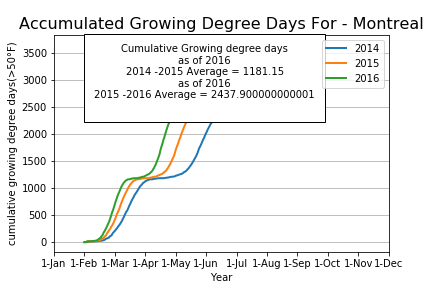
\includegraphics[width=0.8\textwidth]{./docs/MontrealGDD.png} 
\caption{\scriptsize Accumulated GDD for Montreal}
\label{accuGDD_1}		  
\end{figure}

\begin{figure}[!htbp]
\centering
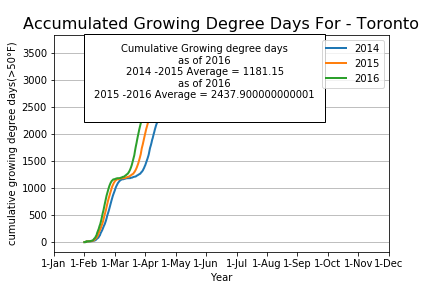
\includegraphics[width=0.8\textwidth]{./docs/TorontoGDD.png} 
\caption{\scriptsize Accumulated GDD for Toronto}
\label{accuGDD_2}		  
\end{figure}
	
\begin{figure}[!htbp]
\centering
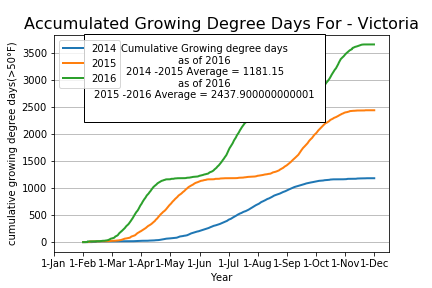
\includegraphics[width=0.8\textwidth]{./docs/VictoriaGDD.png} 
\caption{\scriptsize Accumulated GDD for Victoria}
\label{accuGDD_3}		  
\end{figure}	

\pagebreak 	

\subsection{Task 2.1}
\begin{figure}[!htbp]
\centering
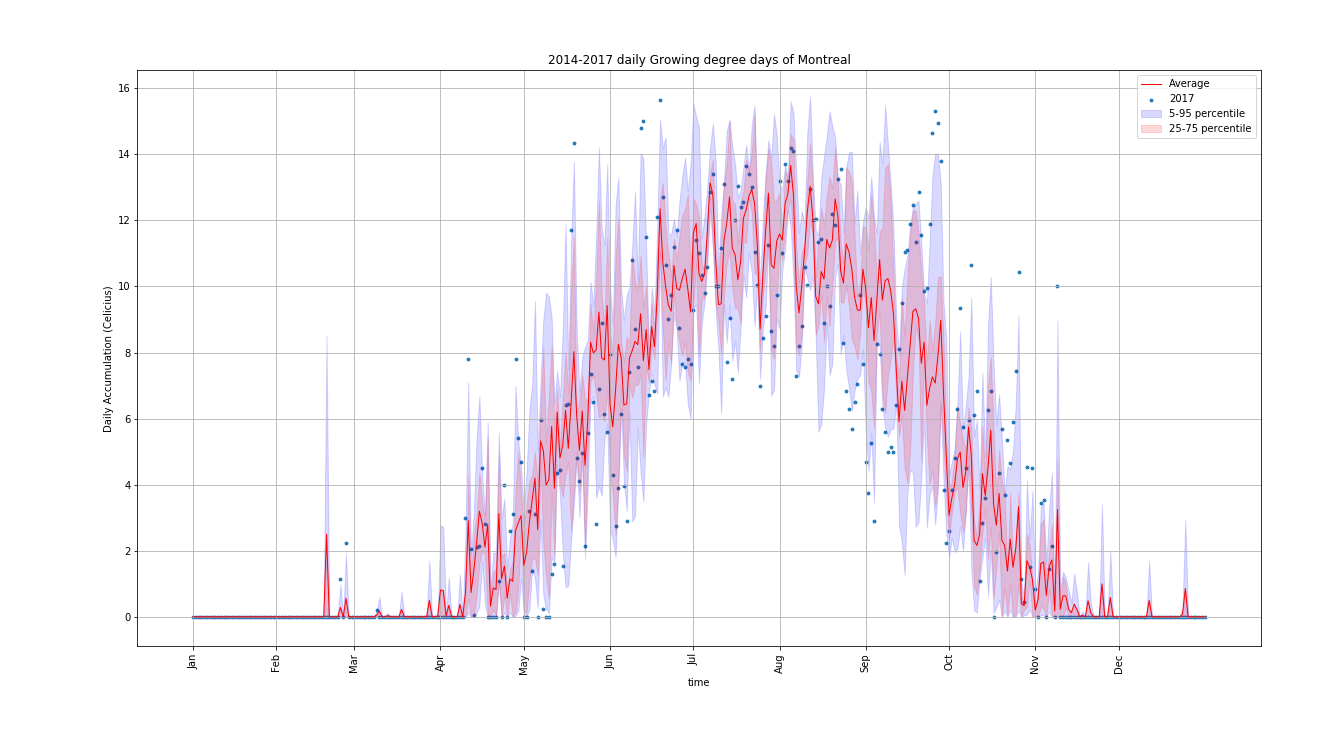
\includegraphics[width=0.8\textwidth]{./docs/task1.png} 
\caption{\scriptsize GDD for Montreal with 5-95\% and 25-75\% percentiles}
\label{GDDwCI}		  
\end{figure}

\pagebreak
\subsection{Task 2.4}
\begin{figure}[!htbp]
\centering
\includegraphics[width=0.8\textwidth]{./montreal_2017.html} 
\caption{\scriptsize Interactive bokeh plot of accumulative GDD for Montreal in 2017}
\label{bokeh}		  
\end{figure}

\pagebreak
\subsection{Task 2.6}
\begin{figure}[!htbp]
\centering
\includegraphics[width=0.8\textwidth]{./docs/LinearReg_city_startyear_endyear.png} 
\caption{\scriptsize Statistical analysis of GDD year-over year for Ottawa}
\label{GDDregression}		  
\end{figure}

\pagebreak


\subsection{Optional Task 1.1}
\begin{figure}[!htbp]
\centering
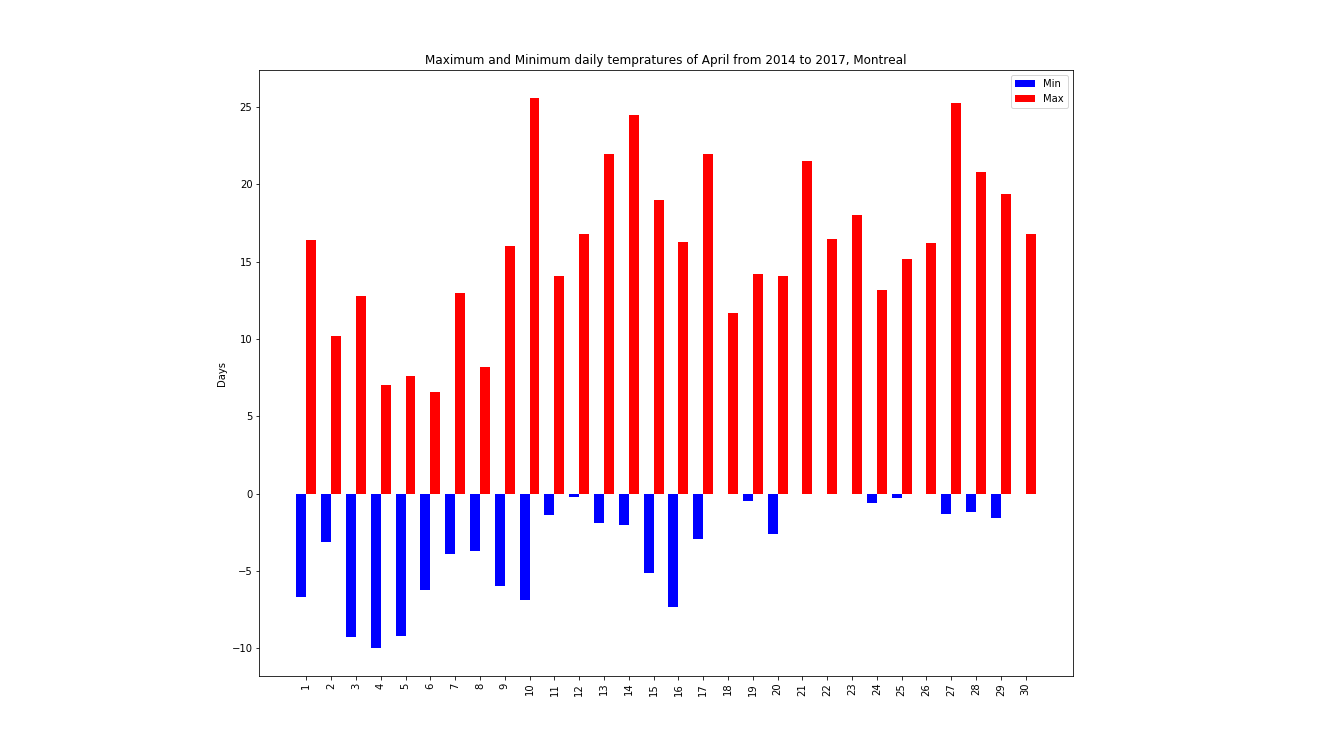
\includegraphics[width=0.8\textwidth]{./docs/aprildaily.png} 
\caption{\scriptsize Maximum and minimum temperatures through the month of April in Montreal}
\label{Aprilmaxmin}		  
\end{figure}

\pagebreak

\subsection{Optional Task 1.2}
\begin{figure}[!htbp]
\centering
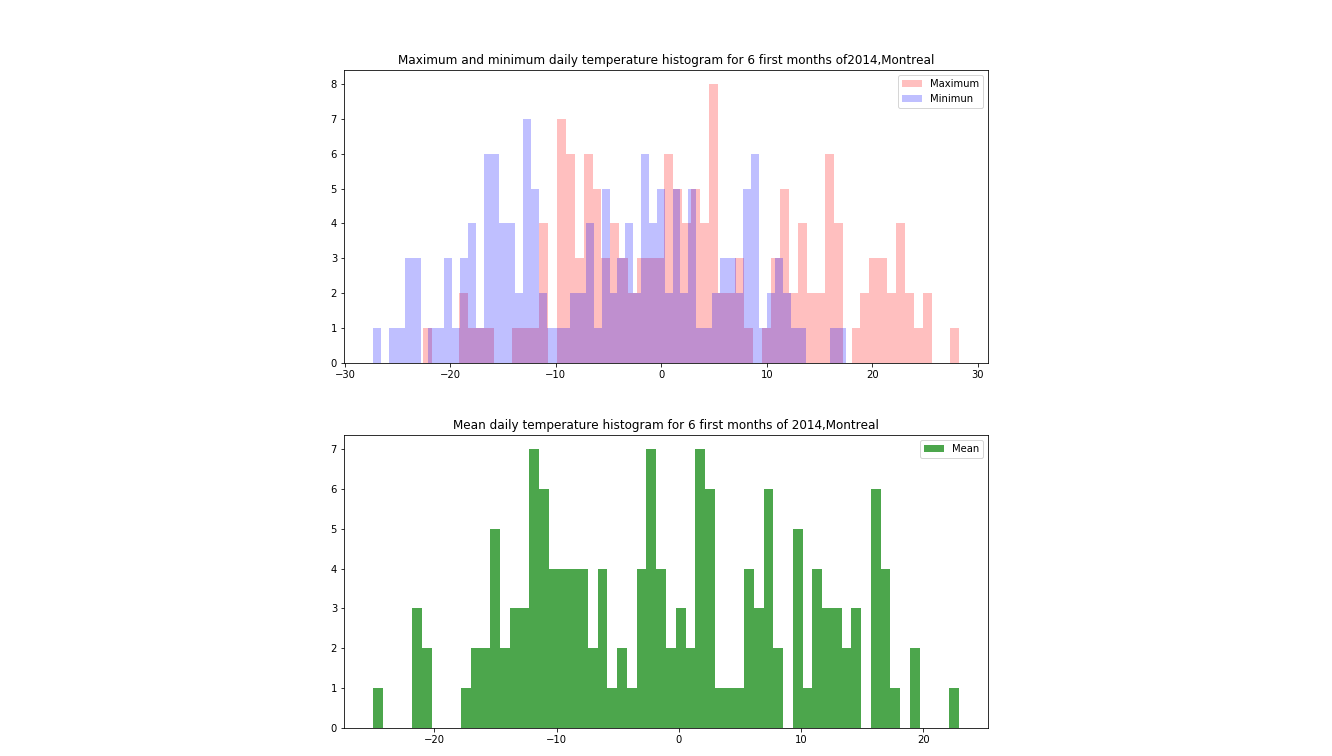
\includegraphics[width=0.8\textwidth]{./docs/histogram2014.png} 
\caption{\scriptsize Histograms of temperature trends in Montreal for 2014}
\label{hist2014}		  
\end{figure}

\begin{figure}[!htbp]
\centering
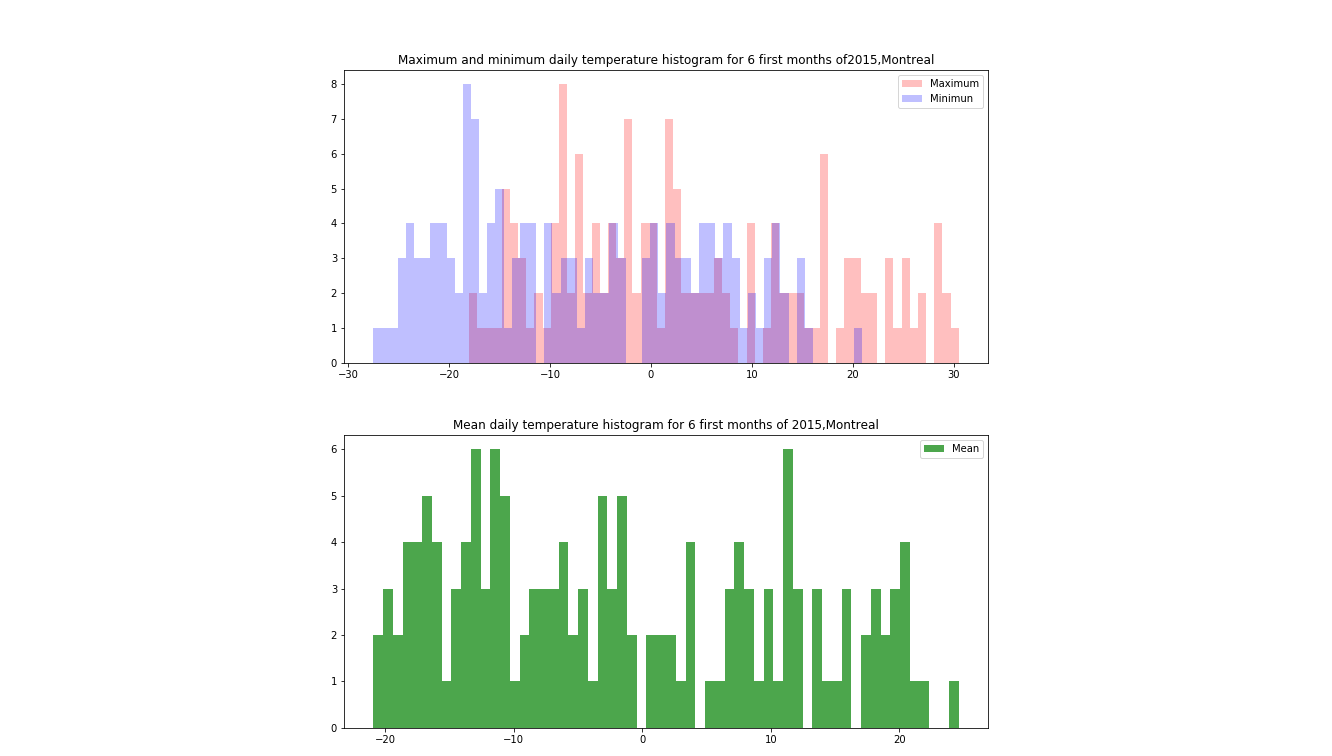
\includegraphics[width=0.8\textwidth]{./docs/histogram2015.png} 
\caption{\scriptsize Histograms of temperature trends in Montreal for 2015}
\label{hist2015}		  
\end{figure}

\begin{figure}[!htbp]
\centering
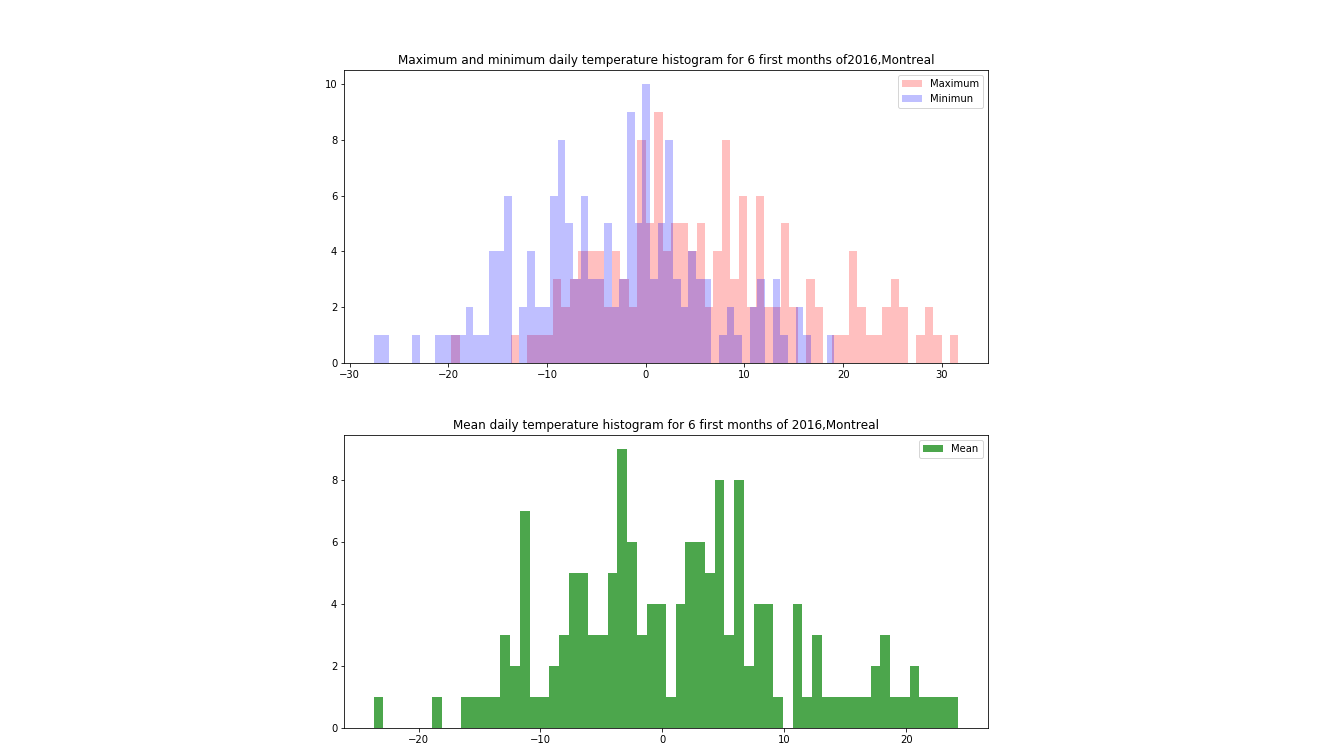
\includegraphics[width=0.8\textwidth]{./docs/histogram2016.png} 
\caption{\scriptsize Histograms of temperature trends in Montreal for 2016}
\label{hist2016}		  
\end{figure}

\begin{figure}[!htbp]
\centering
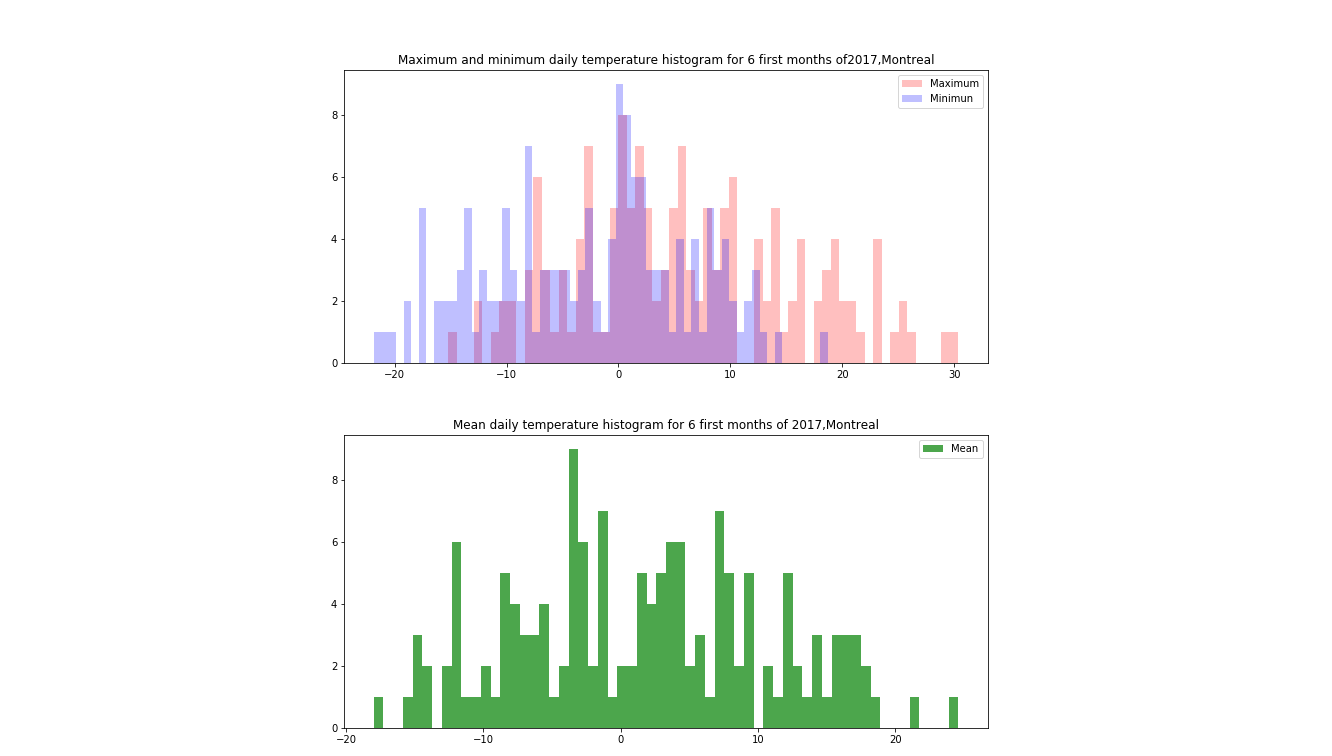
\includegraphics[width=0.8\textwidth]{./docs/histogram2017.png} 
\caption{\scriptsize Histograms of temperature trends in Montreal for 2017}
\label{hist2017}		  
\end{figure}

% % % % % % % % % % % % % % % % % 

\pagebreak

\bibliographystyle{abbrv}
\bibliography{main}

\begin{thebibliography}{2}
\bibitem{GovCan} 
Historical Climate Data | Environment and Climate Change Canada
\\\texttt{http://climate.weather.gc.ca}
\bibitem{GDD MSU} 
Understanding growing degree days | Michigan State University
\\\texttt{http://msue.anr.msu.edu/news/understanding\_growing\_degree\_days}
\bibitem{farmwest} 
Growing Degree Days | Farmwest
\\\texttt{http://www.farmwest.com/node/936}
\end{thebibliography}

\end{document}
